\chapter{Results and Discussion}
The $v_2$ measurement for \pau at \sqsn = 200 GeV 0--5\% centrality completes the set of flow measurements in the small systems available at RHIC: \pau, \dau, and \hau. The goal of this set of measurements is to determine the effect of varying initial collision conditions on the resulting flow.
\section{$v_2$ Measurement}
The resulting $v_2$ measurement for \pau at \sqsn = 200 GeV 0--5\% centrality is shown in Figure \ref{fig:pau_points_alone}. The systematic uncertainty varies from $^{+7.2}_{-13.4}\%$ at low \pt to $^{+7.3}_{-23.8}\%$ at high \pt, where the asymmetric uncertainty is dominated by by non-flow. The fact that the non-flow dominates the systematic uncertainty warrents further discussion on the the treatment of non-flow.
%The systematic uncertainty is very large especially at high \pt and is dominated by non-flow. 

%$^{+7.2}_{-13.4}\%$
%$^{+7.3}_{-23.8}\%$
\begin{figure}[!ht]
\begin{center}
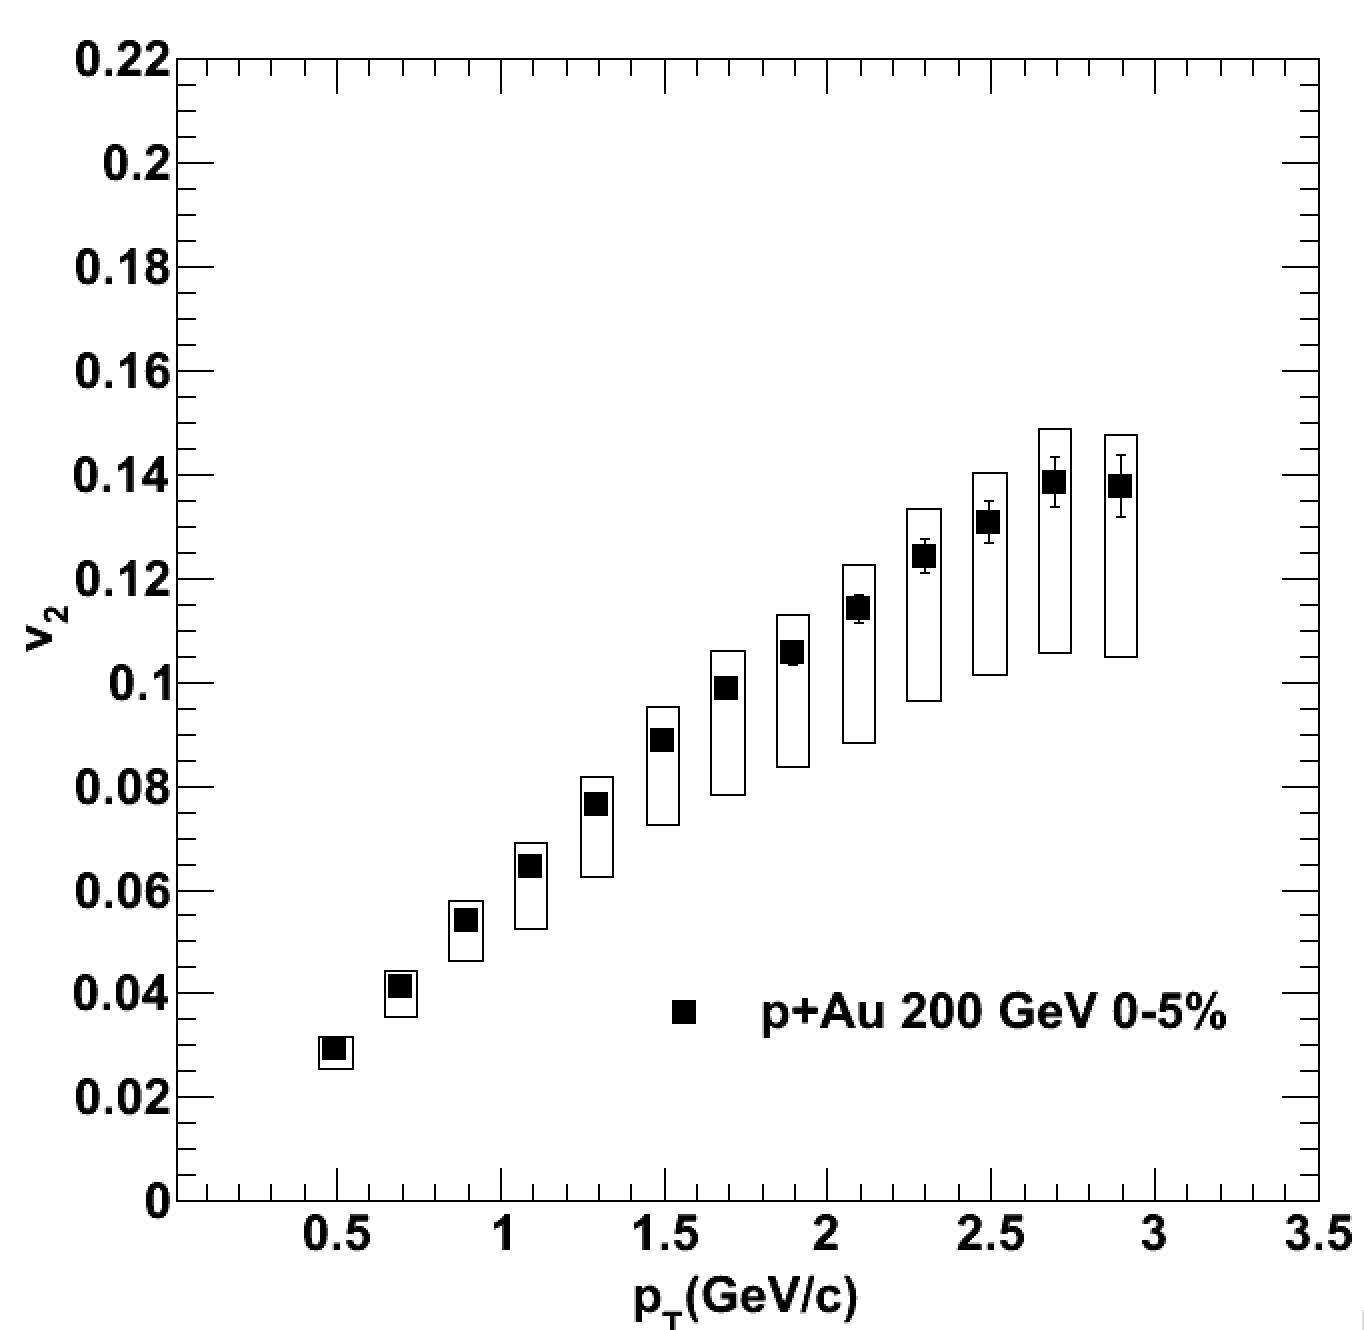
\includegraphics[width=0.65\linewidth]{figs/pau_points.png}
\caption{The $v_2$ measurement of \pau at \sqsn =  200 GeV 0--5\% centrality.}
\label{fig:pau_points_alone}
\end{center}
\end{figure}

\subsection{Non-flow Contribution}
\label{sec:ch5-non-flow}
As was discussed in Section 4.4.2, the non-flow systematic uncertainty can instead be thought of as a systematic error that can be corrected for in our measurement. To further explore this non-flow effect, Figure \ref{fig:pau_points_alone_nf} shows what the \pau measurement looks like by subtracting the  non-flow effect rather than treating it as an uncertainty. Due to non-flow being the dominant source of systematic uncertainty, the corrected \pau points are nearly at the bottom of the systematic uncertainty boxes of the uncorrected points.  The substantial changes this correction makes to the \pau points, especially at high \pt, must be put in context of the field of heavy ion physics. This procedure to estimate the contribution of elementary processes to the measured $v_2$ signal is an attempt at an accurate approximation. Although the non-flow approximation used in this thesis has its merits, there is currently no consensus in the field regarding how to properly quantify how much of the $v_2$ corresponds to ``flow" and how much corresponds to ``non-flow." Other experimental collaborations making flow measurements, such as STAR, ATLAS, and ALICE, treat non-flow in different ways \textbf{to add refs}. Therefore, we chose to explicitly state our methodology to estimate this non-flow and to treat it as a systematic effect that raises the measured $v_2$. %When comparing the \pau points with points from other systems, the non-flow incorporated as a systematic uncertainty.

\begin{figure}[!ht]
\begin{center}
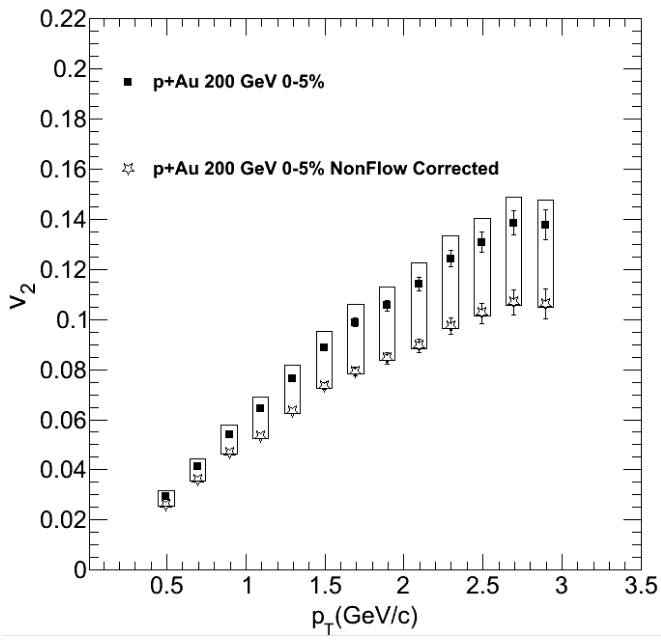
\includegraphics[width=0.65\linewidth]{figs/figure_w_nonflow_corr.png}
\caption{The $v_2$ measurement of \pau at \sqsn =  200 GeV 0--5\% centrality with the statistical and systematic errors corresponding to the bars and the boxes respectively. The stars are the same \pau points but with the non-flow estimate subtracted rather than treated as a systematic uncertainty.}
\label{fig:pau_points_alone_nf}
\end{center}
\end{figure}

%\subsection{$v_2$ vs Multiplicity}
\section{Comparison with Other Species at \sqsn =  200 GeV 0--5\% Centrality}
The substantial $v_2$ in \pau  at \sqsn =  200 GeV is interesting in itself but the significance of the measurement is best understood by comparing it to other small collision system results, specifically \hau~\cite{PhysRevLett.115.142301} and \dau~\cite{PhysRevLett.115.142301} at the same \sqsn energy. In order to properly make the strongest physics statement possible in this comparison, we attempt to hold as many variables constant across all three datasets. Table \ref{tbl:species_compare} compares the various relevant parameters for the three collision species. As shown in the table, the FVTXs was not used in the \dau measurement unlike for the \pau and \hau due to the fact that the FVTX was not installed in 2008 when the \dau measurement was taken. The table also highlights the fact that $dN_{ch}/d\eta$, the $\eta$ dependence of the charged particle multiplicity, has not been measured in \pau \sqsn = 200 GeV, in contrast to \hau and \dau. This fact is relavent because mid-rapidity $dN_{ch}/d\eta$ is an input to the SONIC model for the purposes of multiplicity matching, as discussed in the next section. Among the differences across the columns, the largest is the lack of a non-flow estimate for the \dau dataset. In the interest of measurement compatibility, and for the reason stated in the previous section, there is no non-flow correction applied to any of the datasets.

\begin{table}[h!]
\caption{Dataset Variables Comparison listed in order: center of mass energy per nucleon, centrality, mid-rapidity charged particle multiplicity per unit of psuedo-rapidity from~\cite{PhysRevC.93.024901}, year, trigger (as defined in section \ref{sec:event_plane}) particle sample, trigger particle acceptance, event plane determination, $\Psi_2$ Resolution, condition of available non-flow estimate.}
\begin{center}
    \begin{tabular}{| c | c | c | c |}
    \hline
    Variable & \pau  & \dau & \hau\\ \hline \hline
    \sqsn (GeV) & 200 & 200 & 200\\ \hline
    Centrality &0--5\%  &0--5\% &0--5\% \\ \hline
    Mid-rapidity $dN_{ch}/d\eta$ & N/A & 20.8 $\pm$ 1.5 & 26.3 $\pm$ 1.8 \\ \hline 
    Year (collected) & 2015  & 2008 & 2014 \\ \hline
    Trigger Particle Sample & Charged Hadrons & Charged Hadrons & Charged Hadrons \\ \hline
    Trigger Particle Acceptance & $|\eta| <$ 0.35  & $|\eta| <$ 0.35 & $|\eta| <$ 0.35 \\ \hline
    Event Plane &  -3$<\eta<$-1 (FVTXs) & -3.7$<\eta<$-3.1 (MPCs) &  -3$<\eta<$-1 (FVTXs) \\ \hline
    $\Psi_2$ Resolution & 0.171 & 0.14 & 0.274 \\ \hline %maybe add pt averaged v2?
     Non-flow Estimate& yes & no & yes\\ \hline
     %Glauber $\varepsilon_2$ & 0.23 &  0.54 & 0.50\\ \hline
    \end{tabular}
\end{center}
\label{tbl:species_compare}
\end{table}
%\begin{table}[h!]
%\caption{To Do: make systematic error table.}
%\begin{center}
%    \begin{tabular}{c | c | c | c}
%    \hline
%    variable & \pau  & \dau & \hau\\ \hline \hline
%    \sqsn (GeV) & 200 & 200 & 200\\ \hline
%    \end{tabular}
%\end{center}
%\end{table}
% discuss centrality selections between the different measurements
% maybe show the multiplicity matched plot? would have to accurately explain caveats NO
Figure \ref{fig:v2_3_sys_compare_nohydro} shows the $v_2(\pt)$ measurements in the three systems. All three measurements exhibit substantial $v_2$ values that rise as a function of \pt with a similar shape. Within the error bars of each measurement, the \hau and \dau measurements agree and the \pau measurement is substantially lower. This effect is especially clear at low \pt, where bulk effects would be most dominant. In order to understand the significance of this set of measurements, comparison to standard theoretical models are useful.

\begin{figure}[!ht]
\begin{center}
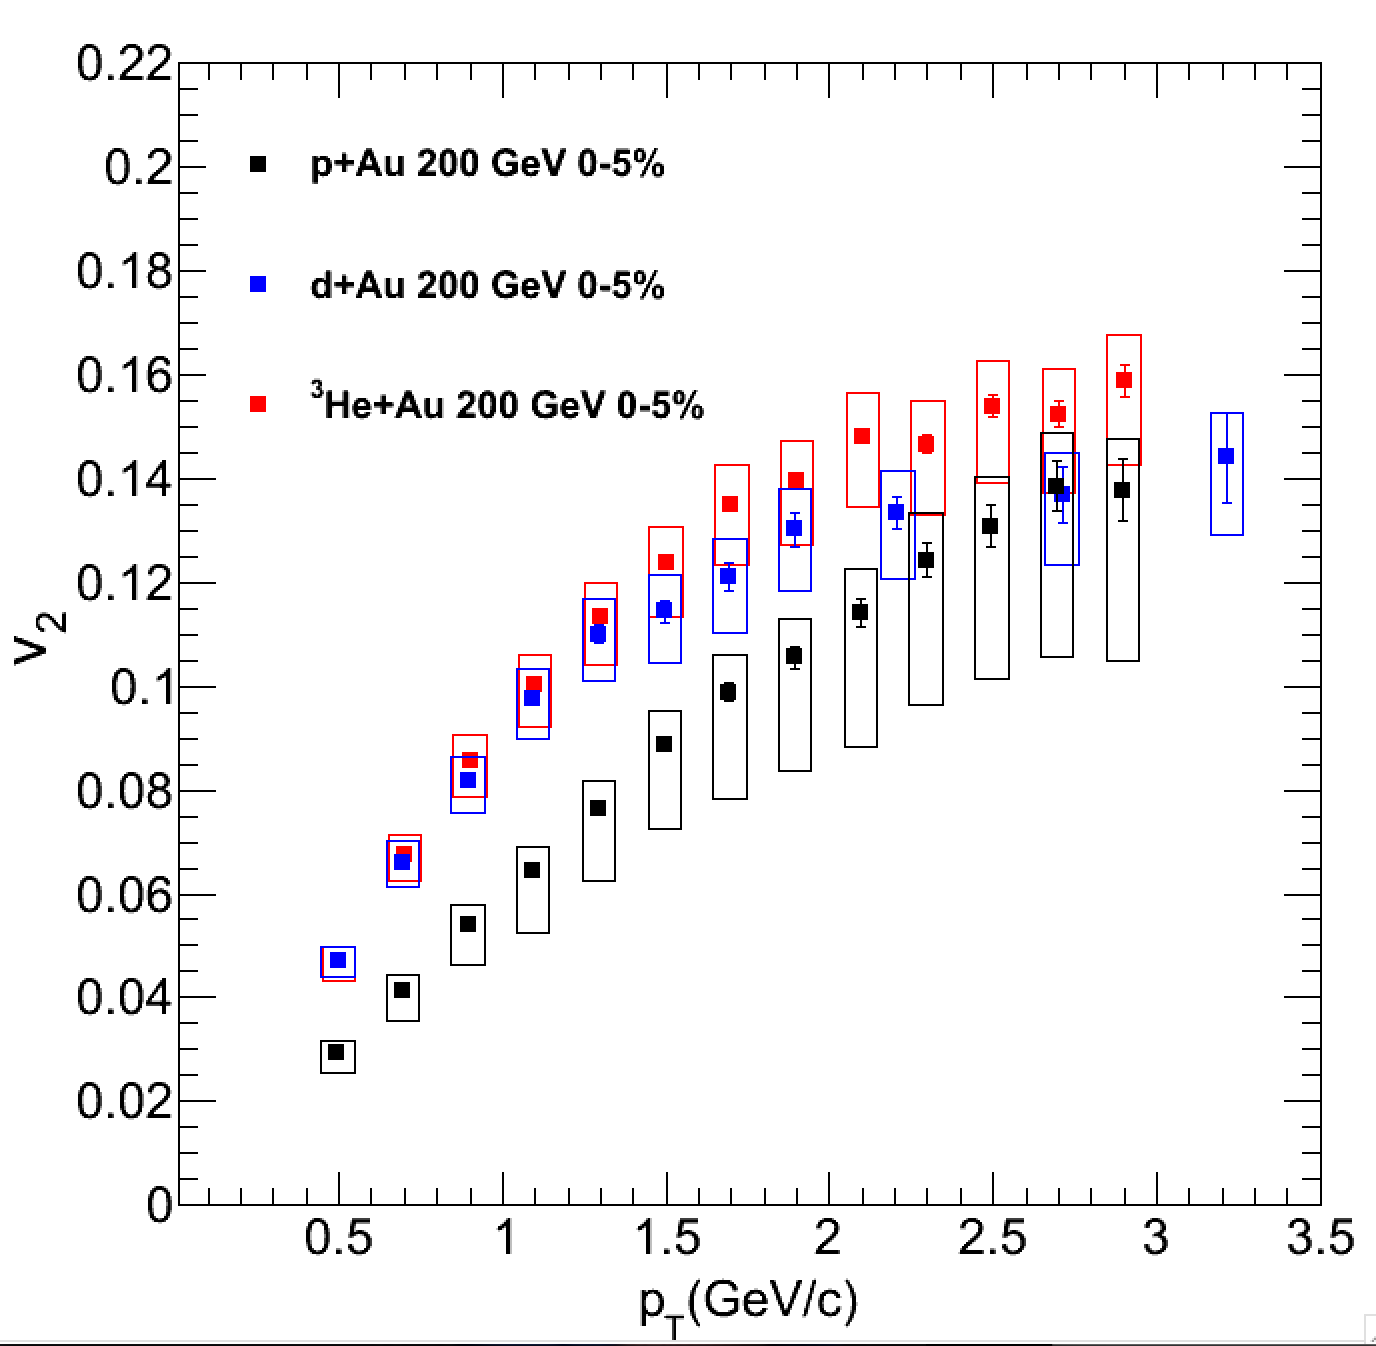
\includegraphics[width=0.65\linewidth]{figs/v2_3_sys_compare_nohydro.png}
\caption{$v_2$ of charged hadrons within $|\eta| <$ 0.35 in 0--5\% \pau compared to calculations using the SONIC model match to the same multiplicity as the data. The model calculations have good agreement with the center of the systematic uncertainty bars.}
\label{fig:v2_3_sys_compare_nohydro}
\end{center}
\end{figure}

\section{Comparison with Theory}
%\subsection{SONIC}
Figure ~\ref{fig:all_system_hydro} shows $v_2(\pt)$ for the three systems and $v_2(\pt)$ calculations for each system from the SONIC hydrodynamic model~\cite{Habich:2014jna}, which incorporates standard Monte Carlo Glauber initial conditions followed by viscous hydrodynamics with $\eta/s=0.08$, and a transition to a hadronic cascade at $T=$ 170 MeV\footnote{Note: please reference Chapter 2 for an in depth discussion about the theoretical models of SONIC, SuperSONIC, IP-Glasma, MC Glauber, and AMPT.}. It is notable that these calculations for each system are matched to the charged particle density at mid-rapidity, with the exact values for 0--5\% centrality of 10.0, 20.0, and 27.0, for \pau, \dau, and \hau collisions, respectively~\cite{Habich:2014jna}. As mentioned above, the $dN_{cn}/d\eta$ has not been measured for \pau, and the value of 10.0 was extrapolated from measurements in the other two systems~\cite{Habich:2014jna}. The SONIC calculation includes both the geometry-related change in the initial conditions and the relative collision multiplicity for the three systems. In all these cases, a good agreement is seen within the systematic uncertainties between the data and the calculation. This agreement between data and hydrodynamic calculation alone strongly supports the notion of initial geometry coupled to the hydrodynamic evolution of the medium as a valid framework to understand small system collectivity.

%\begin{figure}[!ht]
%\begin{center}
%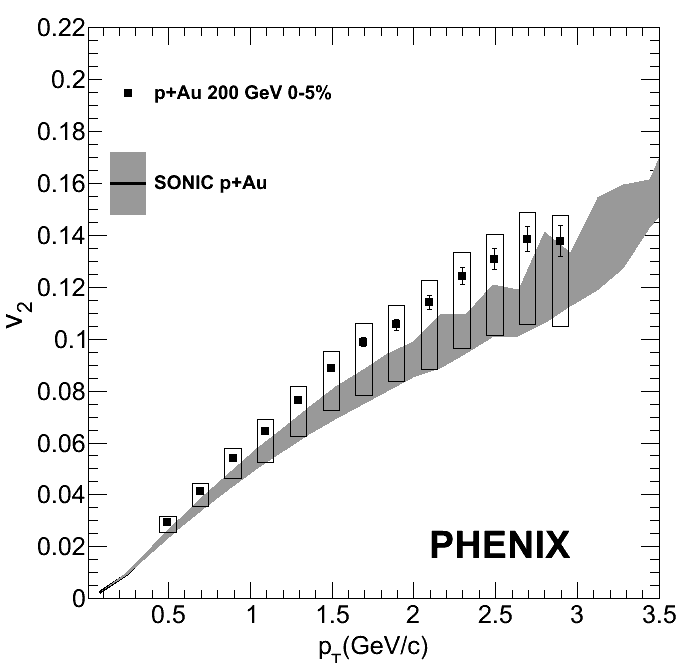
\includegraphics[width=0.65\linewidth]{figs/pau_sonic_alone.png}
%\caption{$v_2$ of charged hadrons within $|\eta| <$ 0.35 in 0\%--5\% \pau compared to calculations using the \textsc{sonic} model match to the same multiplicity as the data. The model calculations have good agreement with the center of the systematic uncertainty bars.}
%\label{fig:hydro_pau_alone}
%\end{center}
%\end{figure}

\begin{figure}[!ht]
\begin{center}
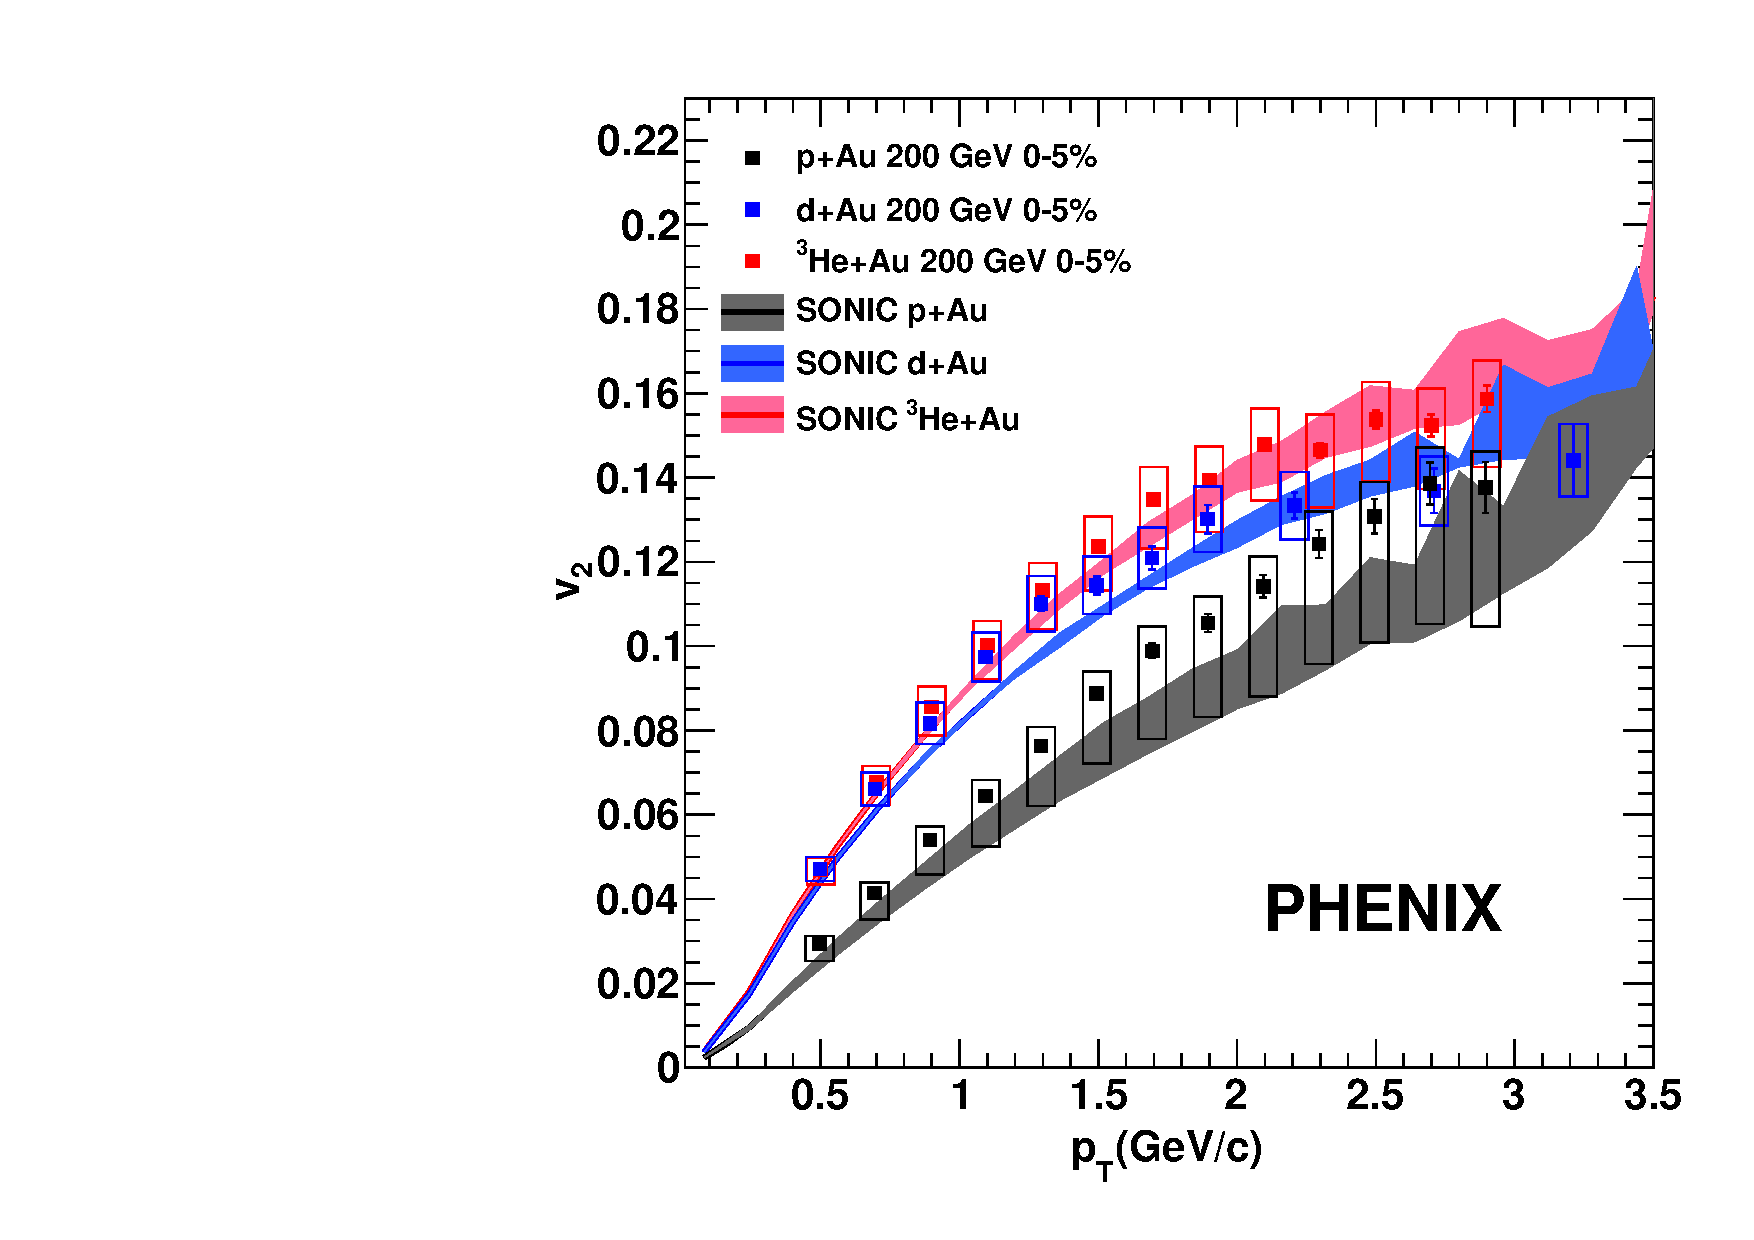
\includegraphics[width=0.65\linewidth]{figs/three_system_comparison_result.png}
\caption{$v_2$ of charged hadrons within $|\eta| <$ 0.35 in 0--5\% \pau, \dau, and \hau central collisions, compared to hydrodynamic calculations using the \textsc{sonic} model, matched to the same multiplicity as the data. Note that the data points shown include non-flow contributions, whose estimated magnitude is accounted for in the asymmetric systematic uncertainties.}
\label{fig:all_system_hydro}
\end{center}
\end{figure}

\subsection{Initial Conditions and Eccentricity}
In order to better understand the comparison of the three systems, a deeper understand of the initial conditions is warranted. One critical quantity to characterize the initial collision symmetry is known as the eccentricity. As mentioned in Chapter 2, the second order eccentricity, $\varepsilon_2$, can be calculated from the distribution of the nucleons involved in the initial collision as:

\begin{equation}
\label{eqn:eccentricity_equation}
\varepsilon_2 = \frac{\sqrt{\langle r^2 \cos(2\phi)\rangle^2+\langle r^2 \sin(2\phi)\rangle^2}}{\langle r^2\rangle},
\end{equation}
where $r$ is the radial nucleon position relative to the centroid of the participants and $\phi$ is the azimuthal angle of the nucleons~\cite{PhysRevC.81.054905}. 

The significance of $\varepsilon_2$ is that $v_2$ should be proportional to $\varepsilon_2$ if the $v_2$ is primarily from elliptical flow. Table \ref{table_geometry_glasma} shows $\varepsilon_2$ calculations from the MC Glauber and IP-Glasma models. The $\varepsilon_2$ values can be understood by looking the top three panels of Figure \ref{fig:initial_condition_comparison} which show the spatial distribution of the energy density of the collisions for the \pau, \dau, and \hau from left to right. It is note worthy that the eccentricities of \dau and \hau collisions are largely based on relative nucleon orientation, where as the initial condition of \pau is solely based on the shape of the lone proton projectile and any fluctuations in the target gold nucleus. Table \ref{tbl:eccentricities} illustrates the uniqueness of the \pau system by showing the diverging values of $\varepsilon_2$ which can be calculated by IP-Glasma and MC Glauber. Unlike MC Glauber, IP-Glasma generates very circular initial conditions for \pau, which correspond to very small $\varepsilon_2$ values. For \dau and \hau, the presence of multiple hot spots wash out differences in single nucleon initial conditions, and thus IP-Glasma and MC-Glauber agree at the 10\% level. 

While the top three panels of Figure \ref{fig:initial_condition_comparison} are example initial energy density distributions for the three systems, the bottom three panels are the system's energy density distributions after a medium has been formed and time evolved hydrodynamically. For the cases of \dau and \hau, the initial hot spot orientation is translated into an inverted orientation. This is due to the fact that the medium is produced with the highest energy density at places where the expanding hotspots overlap. The expanding hotspots create a substantial final state elliptical flow with an event plane angle relative to the spatial orientation of the initial hotspots. For example, in the \dau collision, the event plane vector is transverse to the line that connects the deuteron's nucleons. 

\begin{table}[h!]
\begin{center}
\caption{Initial eccentricity $\varepsilon_2$ of small systems at \sqs = 200 GeV for 0--5\% centrality from Monte Carlo Glauber initial conditions smeared with a two-dimensional Gaussian of width $\sigma=0.4$ fm, and IP-Glasma initial conditions.}
\begin{tabular}{c c c c}
\label{table_geometry_glasma}
 & \pau & \dau & \hau \\ \hline
 Glauber $\langle \varepsilon_2 \rangle$ & $0.23\pm 0.01$ & $0.54\pm 0.04$ & $0.50\pm 0.02$ \\
 IP-Glasma $\langle \varepsilon_2 \rangle$ & $0.10\pm 0.02$ & $0.59\pm 0.01$ & $0.55\pm 0.01$ \\
\label{tbl:eccentricities}
\end{tabular}
\end{center}
\end{table}

\begin{figure}[!ht]
\begin{center}
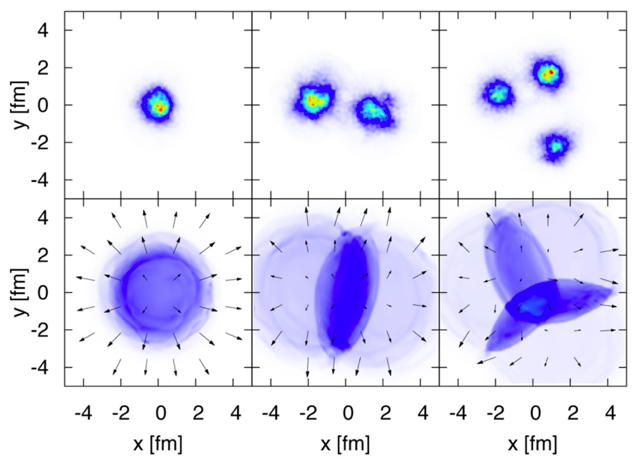
\includegraphics[width=0.75\linewidth]{figs/initial_condition_comparison.png}
\caption{The top three panes show the transverse spatial locations of the initial hot spots of the three collision species, \pau, \dau, and \hau respetively. The bottom three plots show the resulting medium produced from the overlapping hot spots as well as the resulting particle momentum vector field as calculated from a hydrodynamic model, calculation details in ~\cite{Schenke20141039}}
\label{fig:initial_condition_comparison}
\end{center}
\end{figure}

Figure \ref{fig:v2_epsi2_ampt} gives insight into the relation between initial collision eccentricities, as defined in Equation \ref{eqn:eccentricity_equation}, as they are transformed into final state flow. The plot was produced by running many events for \pau, \dau, and \hau systems with different initial spatial distribution smearing (i.e. different $\varepsilon_2$). The final freeze-out hyper-surface of each event is then translated into a distribution of hadrons via the Cooper-Frye freeze-out technique~\cite{PhysRevD.10.186}. Figure \ref{fig:v2_epsi2_ampt} shows the pion $v_2$ at \pt = 1.0 GeV/c divided by $\varepsilon_2$ as a function of $\varepsilon_2$ for each individual \pau, \dau, and \hau event. The figure shows a reasonably common scaling of $v_2/\varepsilon_2$ for all three systems with the \dau and \hau simply extending to larger eccentricities. There are a small set of events with very large $\varepsilon_2$, but have a rather small final $v_2$. Examination of these events reveals them to be \dau events where the two hot spots are so far apart that the hydrodynamic fluids never connect during the time evolution, as seen in the overlay in Figure \ref{fig:v2_epsi2_ampt}, in order to produce nearly any elliptic flow. There are fewer \hau in this category, seen where two nucleons are very close and the third is quite far away, again having the same effect.

\begin{figure}[!ht]
\begin{center}
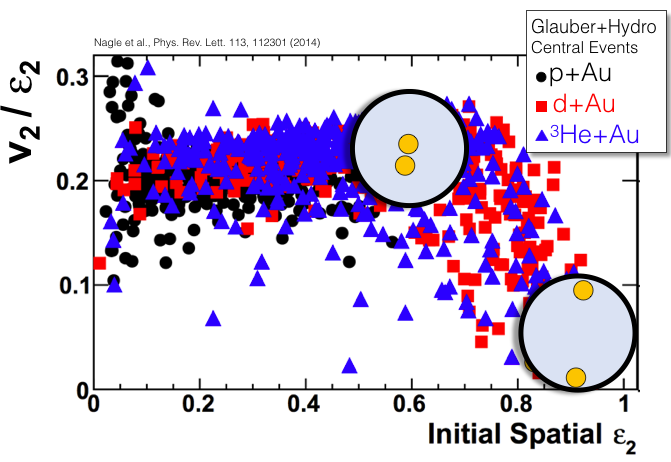
\includegraphics[width=0.6\linewidth]{figs/v2_e2_ampt.png}
\caption{$v_2/\varepsilon_2$ versus $\varepsilon_2$ with the flow coefficient
for pions evaluated at \pt = 1.0 GeV/c from \pau,
\dau, and \hau central (b $<$ 2 fm) events (which roughly corresponds to 0--5\% centrality). The results
are with input parameters $\eta$/s = 1/4$\pi$ and initial Gaussian
smearing $\sigma$ = 0.4 fm and a freeze-out temperatures of $T_F$ = 150
MeV. Diagrams of two possible \dau initial configurations are overlayed on top of the plot. Increasing distance between the two \dau nucleons correspond to a larger $\varepsilon_2$ ~\cite{PhysRevLett.113.112301}.}
\label{fig:v2_epsi2_ampt}
\end{center}
\end{figure}

To further explore the effect of initial conditions on our $v_2$ measurement, we divide the $v_2$ curves by their corresponding $\varepsilon_2$ from Table \ref{table_geometry_glasma}, attempting to establish  a scaling relation between the two quantities. In ideal ($\eta/s=0$) hydrodynamics with long livid systems $v_2$/$\varepsilon_2$ should be independent of $\varepsilon_2$. Figure \ref{fig:v2_divided_epsilon_all_sys} shows that the ratios do not collapse to a common value. As expected, this behavior is also reproduced by the SONIC calculation, because both data and calculation are divided by the same $\varepsilon_2$ values. The lack of scaling in the SONIC calculation can be understood from \dau events where the neutron and proton from the deuteron projectile are far separated and create two hot spots upon impacting the Au nucleus, as seen in Figure \ref{fig:v2_epsi2_ampt}. These events have a large $\varepsilon_2$, but can result in small $v_2$ if the two hot spots evolve separately, never combining within the hydrodynamic time evolution. This effect is present in the \dau and \hau systems, and lowers the average $v_2$/$\varepsilon_2$ as detailed.%add ref?

\begin{figure}[!ht]
\begin{center}
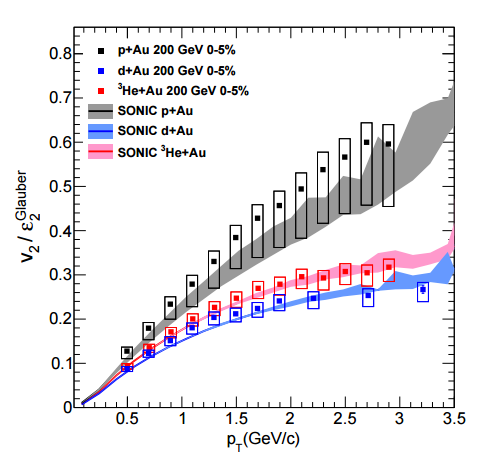
\includegraphics[width=0.65\linewidth]{figs/v2_divided_epsilon_all_sys.PNG}
\caption{$v_2$ of charged hadrons within $|\eta|$ $<$ 0.35 in 0--5\% \pau,  \dau, and \hau central collisions, divided by their corresponding eccentricity $\varepsilon_2$ from Glauber calculations, compared to SONIC calculations of the same quantity. Note that the data points shown include non-flow contributions, whose estimated magnitude is accounted for in the asymmetric systematic uncertainties.}
\label{fig:v2_divided_epsilon_all_sys}
\end{center}
\end{figure}

Although, MC Glauber and IP-Glasma are the established models for calculating initial conditions in this context, new models for calculating the initial conditions are promising. A model for initial conditions which incorporates more degrees of freedom by extending the Monte Carlo Glauber approach to also incorporate collisions between constituent quarks, basically increasing the granularity of the simulation ~\cite{PhysRevC.67.064905}. In the rightmost panel of Figure \ref{fig:epsilon_2_theory}, the initial eccentricities $\varepsilon_2$ in \pau, \dau, and \hau obtained by incorporating constituent quarks, in addition to multiplicity fluctuations, are found to be $\varepsilon_2$ = 0.42, 0.54, and 0.54, respectively. This calculation assumes a Gaussian density distribution of low-x gluons around each constituent quark, of width $\sigma_g$ = 0.3 fm. The $\varepsilon_2$ of \dau and \hau systems show minimal sensitivity to the incorporation of constituent quarks and multiplicity fluctuations. However, \pau has a substantially larger $\varepsilon_2$ than in the models shown in Table \ref{tbl:eccentricities} when incorporating these effects. Another attempt at the calculation incorporating constituent quarks and multiplicity presents calculations in which case a lower $\varepsilon_2$ = 0.34 is obtained for \pau ~\cite{PhysRevC.94.024919}. This result shows that when compared to the Glauber $\varepsilon_2$ for \pau in Table \ref{tbl:eccentricities}, quark-level degrees of freedom and multiplicity fluctuations may both play a significant role. In addition to the constituent MC Glauber, it is worth mentioning that an intriguing method for understanding the initial conditions in \pau comes from fluctuations of the shape of the proton, as described in Ref. ~\cite{Schlichting2014313}. 

\begin{figure}[!ht]
\begin{center}
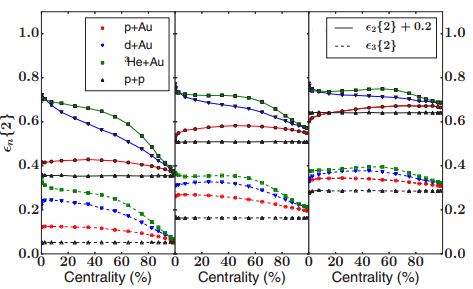
\includegraphics[width=0.6\linewidth]{figs/theoretical_epsilon_values.png}
\caption{Centrality dependence of $\varepsilon_2$ calculated in a variety of small collision systems with a variety of models for collision detection [disklike (left), Gaussian (middle), quark-subdivided nucleons with $\sigma_g$ = 0.3 fm (right)]~\cite{PhysRevC.94.024919}.}
\label{fig:epsilon_2_theory}
\end{center}
\end{figure}

\subsection{Comparison to Alternative Models}%reword section to avoid possible plagiarism
Although hydrodynamic models like SONIC, which incorporate MC Glauber plus relativistic hydrodynamics, are the standard in which elliptical flow is understood in the field of heavy ions, it is important to test the consistency of other models with our data. Figure \ref{fig:indepth_comp_three} depicts the measured $v_2(\pt)$ data curves with four different model comparisons. Theoretical predictions are available in the literature, most notably from hydrodynamics with Glauber initial conditions (SONIC ~\cite{Habich2015} and SuperSONIC ~\cite{Romatschke2015}), hydrodynamics with IP-Glasma initial conditions \cite{Schenke20141039}, and A-Multi-Phase-Transport Model (AMPT) ~\cite{PhysRevC.72.064901}. The SuperSONIC model uses the same technique for initial conditions, hydrodynamic expansion, and hadronic cascade as SONIC, yet additionally incorporates pre-equilibrium dynamics with a calculation in the framework of the AdS/CFT correspondence ~\cite{PhysRevLett.111.222302}.

As mentioned in Chapter 2, calculations using IP-Glasma initial conditions followed by viscous hydrodynamics have been successfully used to describe collectivity in A+A collisions, so it is reasonable to apply IP-Glasma to $v_2$ in small systems. For the model of IP-Glasma+Hydro, in the case of \dau and \hau, a better agreement with data can be achieved by increasing the value of $\eta$/s or by including a hadronic cascade stage. However, doing so would lower the prediction for \pau even further. This demonstrates that IP-Glasma does not generate the appropriate initial conditions to account for measured $v_2$ via hydrodynamic flow.

SONIC and SuperSONIC both agree well with the data of all three systems, although the agreement with the \pau points only agrees within in the large systematic uncertainty bars. As mentioned above, the agreement of hydrodynamic models supports the idea of initial geometry as the driver of the $v_2$ signal. Additionally, the three different initial geometries provided by the datasets are useful in constraining the parameters in the SONIC and SuperSONIC models such as $\eta$/s, the transition temperature to a hadron cascade, and the Monte Carlo Glauber smearing of nucleon coordinates of $\sigma$ = 0.4 fm.

Finally, AMPT, as described in Chapter 2, combines partonic and hadronic scattering in a single model. Central AMPT events with impact parameter $b<2$ have a midrapidity $dN_{ch}/d\eta$ = 8.1, 14.8, and 20.7 for \pau, \dau, and \hau, respectively. AMPT uses the same Monte Carlo Glauber initial conditions used to characterize event geometry as in SONIC or SuperSONIC. However, AMPT makes use of the initial Glauber geometry information to compute $v_2$ relative to the participant plane~\cite{PhysRevC.92.054903}. AMPT yields results that agree reasonably well with the data below \pt $\approx$ 1 GeV/c, yet under predict them at higher \pt. Although AMPT does not describe the data as well as SONIC, AMPT has successfully been applied to a variety of systems at RHIC and the LHC~\cite{PhysRevC.93.054911}. 
%See, for example, \textbf{add refs}. 
%Refs.~\cite{Adare:2015cpn,Koop:2015wea,Ma:2016fve,ma_long-range_2014,ma_long-range_2014}

%\subsection{IP-Glasma with Hydro}
\begin{figure}[!ht]
\begin{center}
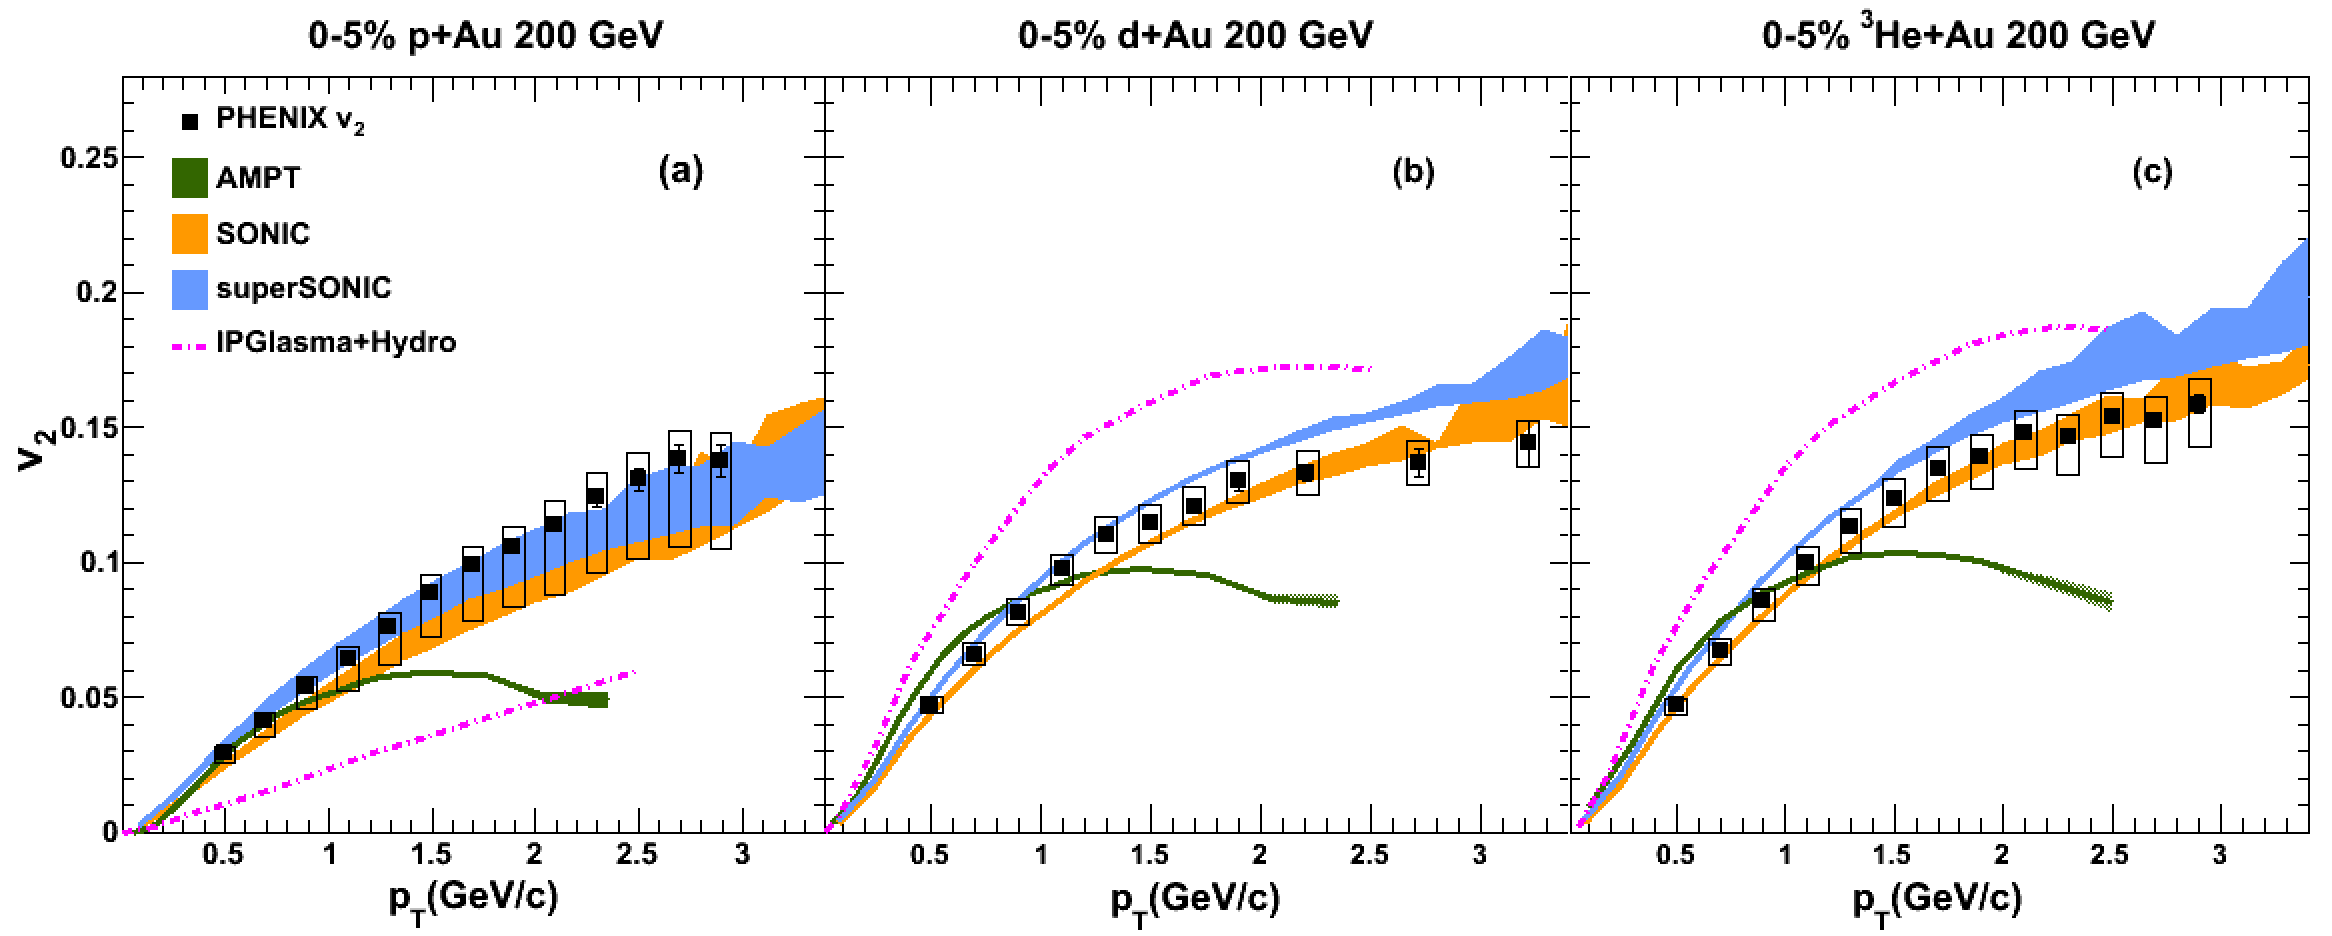
\includegraphics[width=1.0\linewidth]{figs/indepth_theory_comparison.png}
\caption{Transverse momentum dependence of $v_2$ in central 0--5\% (a) \pau, (b) \dau, and (c) \hau collisions at \sqsn = 200 GeV. Theoretical calculations from AMPT, SuperSONIC, and IP-Glasma+Hydro are shown in each panel. Note that the data points shown include non-flow contributions, whose estimated magnitude is accounted for in the asymmetric systematic uncertainties.}
\label{fig:indepth_comp_three}
\end{center}
\end{figure}

